\documentclass{article}
\usepackage[utf8]{inputenc}
\usepackage[a4paper, margin=1in]{geometry}
\usepackage{siunitx}
\usepackage{amsmath}
\usepackage{enumitem}
\usepackage{esdiff}
\usepackage{pgfplots}
\usepackage{listings}
\usepackage{xcolor}

\pgfplotsset{compat=1.18, width=10cm}

\tolerance=1
\emergencystretch=\maxdimen
\hyphenpenalty=10000
\hbadness=10000

\sisetup{
    input-ignore={.},
    output-decimal-marker={,},
    group-minimum-digits=4,
    group-separator={.},
    group-digits=integer
}

\definecolor{darkgray}{rgb}{.4,.4,.4}

\lstdefinestyle{code}{
    aboveskip={1.3\baselineskip},
    basicstyle=\normalsize\ttfamily\linespread{4},
    breaklines=false,
    columns=fullflexible,
    commentstyle=\color[rgb]{0.127,0.427,0.514}\ttfamily\itshape,
    escapechar=@,
    extendedchars=true,
    frame=single,
    identifierstyle=\color{black},
    inputencoding=latin1,
    keywordstyle=\color[HTML]{228B22}\bfseries,
    ndkeywordstyle=\color[HTML]{228B22}\bfseries,
    numbers=left,
    numberstyle=\normalsize,
    prebreak = \raisebox{0ex}[0ex][0ex]{\ensuremath{\hookleftarrow}},
    stringstyle=\color[rgb]{0.639,0.082,0.082}\ttfamily,
    upquote=true,
    showstringspaces=false,
    xleftmargin=5ex,
    aboveskip=5pt
}

\newcommand{\penyelesaian}{\textbf{Penyelesaian: }}

\title{\textbf{Komputasi Numerik: Tugas x}}
\author{Kelompok 15}
\date{}

\begin{document}

\maketitle

\begin{enumerate}
    \item Soal 1 \\
    \penyelesaian Penyelesaian soal 1

    \item Soal beranak
    \begin{enumerate}
        \item Subsoal (a) \\
        \penyelesaian Penyelesaian soal 1 subsoal (a)

        \item Subsoal (b) \\
        \penyelesaian Penyelesaian soal 1 subsoal (b)

        \item Subsoal (c) \\
        \penyelesaian  Penyelesaian soal 1 subsoal (c)
    \end{enumerate}

    \item Soal grafik \\
    \penyelesaian \\
    \begin{center}
        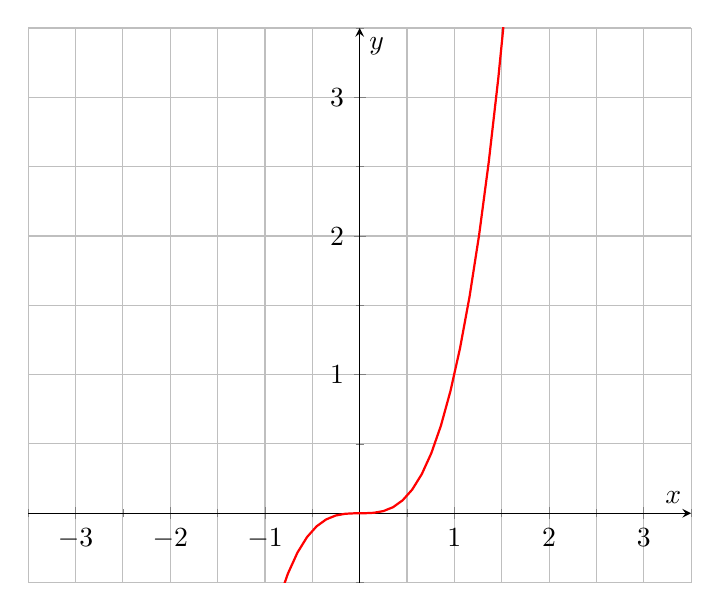
\begin{tikzpicture}
            \begin{axis}[grid=both,ymin=-0.5,ymax=3.5,xmax=3.5,xmin=-3.5,
                        minor tick num=1,axis lines = middle,xlabel=$x$,ylabel=$y$]
                \addplot[color=red, thick, samples=100]{x^3};
            \end{axis}
        \end{tikzpicture}
    \end{center}

    \item Soal algoritma \\
    \penyelesaian
    \begin{lstlisting}[style=code,language=c]
#include <iostream>

int main() {
    printf("Hello World!");

        return 0;
}
    \end{lstlisting}
\end{enumerate}

\end{document}